
\chapter{Tracking usage parameters}
While answering the question, users certain usage attributes are logged automatically in every 5 seconds. There are 17 attributes that are logged. The attributes are average mouse left click, average mouse right click, average mouse double click, average mouse scroll, average cursor x-distance, average cursor y-distance, average key down to up time, average key up to down time, average key down to down time, average regular key press, average enter key press, average arrow key press, average backspace key press, average function key press etc. We also collected some meta data from the user. These are the name, age, occupation and birth year of the survey participant.

\begin{figure}
\centering
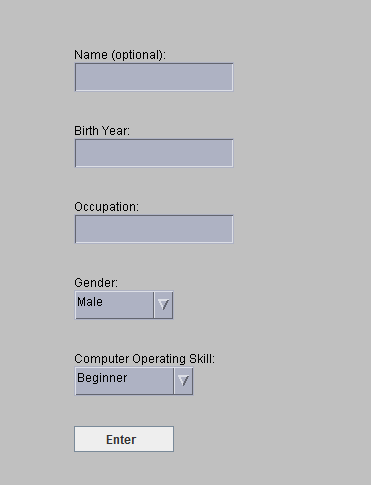
\includegraphics[width=3in,clip,keepaspectratio]{Chapters/figures/startPageSurvey.png}
\caption{Start page of the survey}
\label{Optional }
\end{figure}

\begin{figure}
\centering
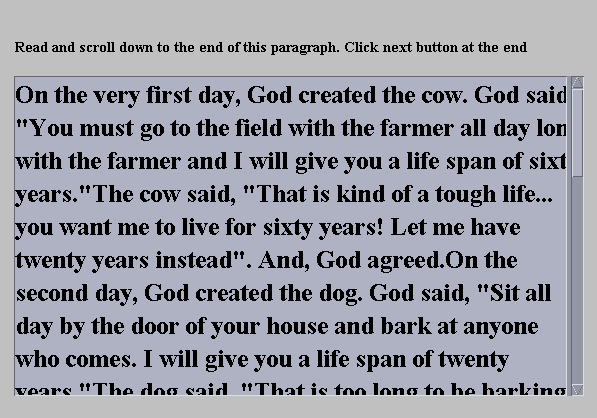
\includegraphics[width=2.5in,clip,keepaspectratio]{Chapters/figures/scrollText.png}
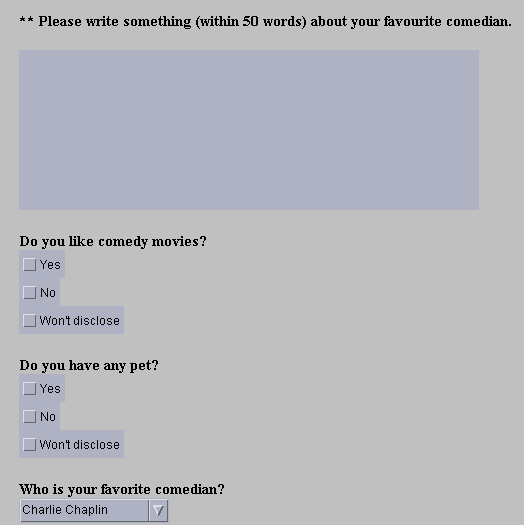
\includegraphics[width=2.5in,clip,keepaspectratio]{Chapters/figures/survey.png}
\caption{Text and various questions to capture scrolling and other usage attributes}
\label{Optional2 }
\end{figure}

